\section{Step size adjustment ability estimation}
\label{sec:eval-stepsize}

From the previous experiment in Section~\ref{sec:eval-rasch}, it is evident that calibrating the entire item bank takes a long time.
Similarly, computing the ability estimate based on the entire response pattern of a user takes too long.
Currently, about 15,000 challenges are completed every day, that is about one challenge every five seconds and this number is only expected to go up.
The computations to estimate the ability of a single user easily exceed that.
For a procedure that has to be executed this frequently, even a minute is too long.

\subsection{Goals and research questions}
The main \textit{goal} of this experiment is to evaluate different approximation procedures for the ability estimates.
The \textit{purpose} is to determine if they can be used to improve the efficiency of the ability computations without a significant loss in accuracy.
The \textit{quality focus} is the accuracy of the procedures with increasing numbers of answered items.
The above goal can be achieved by means of an experiment aimed at answering the following question for each procedure:
\begin{itemize}
    \item \textbf{Q1} how big is the mean error of the approximation after every 5 challenges?
\end{itemize}

\subsection{Approximation procedures}
In research literature, I have found two so-called step size adjustment procedures that are used in \glspl{cat}.
These procedures update the latest estimate based on either a fixed or variable step size~\cite{dodd1995computerized}.

\paragraph{Fixed step size} With a fixed step size, the ability estimate is increased (or decreased) by a specific amount, often between 0.4 and 0.7, when the user answers an item correctly (or incorrectly).
In this experiment the smallest step size of 0.4 is used for the evaluation.

\paragraph{Variable step size} With a variable step size the new ability estimate is placed at the halfway point between the current estimate and the difficulty of one of the two most extreme items in the item bank.
This is possible because the calibration techniques of \gls{irt} place users and items on the same scale.
If the user answers an item correctly, then the highest item parameter is used, if not, the lowest is used.
This procedure makes sense when one considers that the item selection algorithm in \glspl{cat} continuously selects items that are significantly above the current estimated ability level of the user, as explained in Section~\ref{sec:cf-alternatives}.
This is not the case for the historical data, and will also not be the case for the item selection of the \gls{its} in the future.
With more forgiving item selection this procedure will likely become inaccurate over time.

\paragraph{Adaptive step size} As an improvement, I have developed a variation of this procedure that uses the difficulty of the selected item instead of the difficulty of the extreme items in the item bank.
This adaptive step size procedure is shown in Algorithm~\ref{al:stepsize}.
When the user answers an item correctly that was expected to be hard, the ability estimate is increased to the halfway point between this item and the current estimate.
Similarly, when the user answers an item incorrectly that was expected to be easy, the ability estimate is decreased to the halfway point.

In the other cases, the outcome of the answer confirms that the current ability estimate is accurate.
A question that is more difficult than the user's current ability level is answered incorrectly, or a question below the ability level is answer correctly.
The player can then optionally be rewarded or punished with a fixed value, similar to the fixed step size adjustment procedure.
For this experiment, two variations of the adaptive step size procedure are tested, one with a fixed reward of 0.2 and one without a fixed reward.

\begin{algorithm}[H]
\SetAlgoLined
\SetKwInOut{Input}{input}
\SetKwInOut{Output}{output}
\Input{user ability $\bm\theta_i$\\ item difficulty $\beta_j$ \\ answer $X_{ij}$ \\an optional punishment/reward value $r$}
\Output{updated user ability $\bm\theta_i$}
    \uIf{$X_{ij}$ is correct}{
        \uIf{$\bm\theta_i \leq \beta_j$}{return ($\bm\theta_i$ + $\beta_j$)/2}
        \Else{return $\bm\theta_i$ + $r$}
    }
    \Else{
        \uIf{$\bm\theta_i \geq \beta_j$}{return ($\bm\theta_i$ + $\beta_j$)/2}
        \Else{return $\bm\theta_i$ - $r$}
    }
\caption{\label{al:stepsize}Adaptive step size adjustment procedure}
\end{algorithm}

\subsection{Experimental set-up}
The different procedures are evaluated by comparing their approximations with the (accurate) estimated \gls{irt} ability.
To do this, an \gls{irt} ability estimate is needed for each user at each point in time, which requires many long-running \gls{irt} calibration procedures.
The five frameworks with the most data were chosen to use in the evaluation.
These are Java Spring, Java \gls{ee}, NodeJS Express, Pseudocode and Python Django.
The \gls{irt} ability was estimated for every user after every 5 completed challenges.

Each of the four procedures starts from the \gls{irt} ability estimate after 20 completed challenges.
From that point forward, the approximation methods are applied to the outcome of each challenge attempt.
The resulting approximations are compared to the \gls{irt} ability after every 5 challenges.

\subsection{Findings}
For each approximation method, the evolution of the mean error as a percent of the full ability scale, is shown Figure~\ref{fig:stepsize}.
The fixed step size adjustment becomes excessively inaccurate after only 15 to 20 challenges following the initial calibration.
After 200 challenges, the mean error of this approximation is up to 300\%.
While the adaptive step size procedure with a fixed reward is significantly better, its error still becomes excessively large and rises indefinitely.
The seemingly ever increasing error for these two procedures is explained by the large amount of users who play challenges that are below their skill level, and hence often answer them correctly.
With these two procedures, the ability level of users like this is increased each time, while these answers have no significant impact on the accurate estimates.

This effect is still visible for the variable step size adjustment procedure.
However, with this procedure the estimate does not exceed the difficulty of the most difficult item in the item bank, which limits the error to about 30\%.

The adaptive step size procedure without reward or punishment is the most accurate.
With this procedure, the ability estimate is not adjusted if the outcome of an item is as expected according to the current estimate.
The ability estimates of users who are answering easy items correctly is not updated.
For correct answers to difficult challenges or for incorrect answers to easy challenges, the estimate is moved in the right direction, but using smaller steps than the variable step size procedure.
The mean error of 10\% is acceptable for it to be used in the \gls{its}, as will become evident in a following experiment in Section~\ref{sec:eval-learning}.
This implies that the full calibration procedure is only necessary once, for the initial calibration.
In practice, the abilities for existing users will still periodically be re-calibrated along with the initial calibration of new users.

\begin{figure}
    \centering
    %\input{03-education/plots/stepsize}
    \includegraphics[page=13]{03-education/figures/tikzfigures.pdf}
    \caption[Error rates of step size adjustment procedures]{The error rates of the two procedures with a fixed step or a fixed reward become excessively large. For the variable step size procedure, the error rate is capped at around 30\%. The adaptive step size procedure without fixed reward is the most accurate and its error rate does not exceed 10\%.}
    \label{fig:stepsize}
\end{figure}
